% +------------------------------------------------------------------------+
% | Reference manual page: Triangulation_cw_ccw_2.tex
% +------------------------------------------------------------------------+
% | 29.03.2000   Mariette Yvinec
% | Package: Triangulation
% | 
\RCSdef{\RCSTriangulationcwccwRev}{$Revision$}
\RCSdefDate{\RCSTriangulationcwccwDate}{$Date$}
% |
%%RefPage: end of header, begin of main body
% +------------------------------------------------------------------------+


\begin{ccRefClass}{Triangulation_cw_ccw_2}  %% add template arg's if necessary

%% \ccHtmlCrossLink{}     %% add further rules for cross referencing links
%% \ccHtmlIndexC[class]{} %% add further index entries

\ccDefinition
  
The class \ccRefName\ 
offer  two functions \ccStyle{int cw(int i)} and 
\ccStyle{int ccw(int i)} 
which given the index of a vertex in a face
compute the index of the next vertex  of the same face
in clockwise
or counterclockwise order.
This works also for neighbor indexes.
 Thus, for example the neighbor 
\ccc{neighbor(cw(i))} of a face \ccc{f} is
 the
neighbor  which is next to \ccc{neighbor(i)} turning clockwise
around \ccc{f}. The face \ccc{neighbor(cw(i))}
is also the first face encountered after \ccc{f} when
turning clockwise around vertex \ccc{i}
of~\ccc{f}.

Many of the classes in the triangulation package
inherit from \ccRefName. This is for instance the case for
\ccc{CGAL::Triangulation_2<Traits,Tds>::Face}.
 Thus, for example the neighbor 
\ccc{neighbor(cw(i))} of a face \ccc{f} is
 the
neighbor  which is next to \ccc{neighbor(i)} turning clockwise
around \ccc{f}. The face \ccc{neighbor(cw(i))}
is also the first face encountered after \ccc{f} when
turning clockwise around vertex \ccc{i}
of~\ccc{f}.



 \begin{figure}
\begin{ccTexOnly}
    \begin{center}
     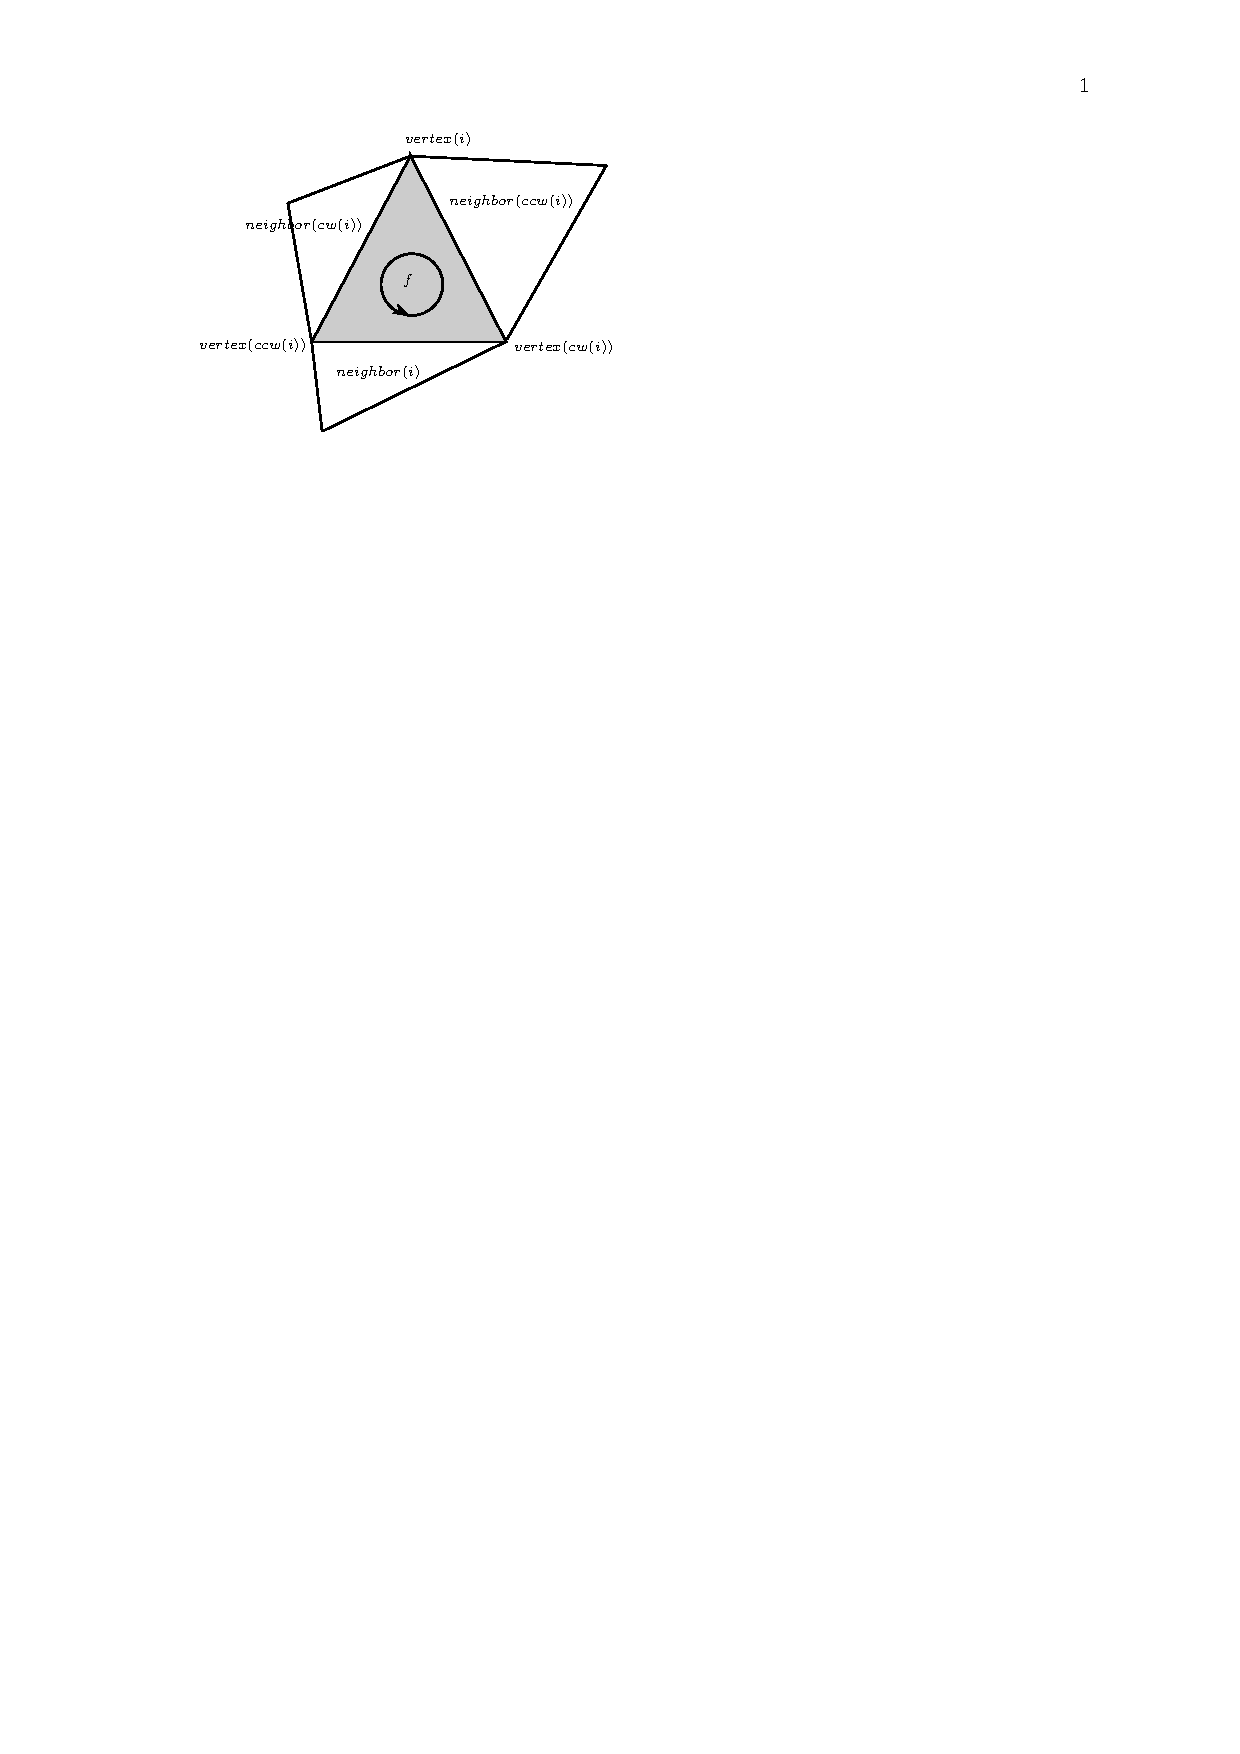
\includegraphics{Triangulation_2/neighbors}
    \end{center}
\end{ccTexOnly} 
    \caption{Vertices and neighbors.
    \label{Triangulation_ref_Fig_neighbors_bis}}
  \begin{ccHtmlOnly}
<CENTER>
<img border=0 src="./neighbors.gif" align=center alt="Neighbors">
</CENTER>
\end{ccHtmlOnly} 
\end{figure}

\ccInclude{CGAL/Triangulation_2.h}



\ccCreation
\ccCreationVariable{a}  %% choose variable name

\ccConstructor{Triangulation_cw_ccw_2();}{default constructor.}

\ccOperations
\ccMethod{int ccw(const int i) const;}
{returns the index of the  neighbor or vertex that is  next to 
the neighbor or vertex with index \ccc{i}
in counterclockwise order around a face.}
\ccGlue
\ccMethod{int cw(const int i) const;}
{returns the index of the  neighbor or vertex that is  next to 
the neighbor or vertex with index \ccc{i}
in counterclockwise order around a face.}

\ccSeeAlso
\ccc{CGAL::Triangulation_2<Traits,Tds>} \\
\ccc{CGAL::TriangulationDSFace_2} \\

\end{ccRefClass}

% +------------------------------------------------------------------------+
%%RefPage: end of main body, begin of footer
% EOF
% +------------------------------------------------------------------------+

